\section{Data generation}

\begin{definition}[\textit{Synthetic data}]
    Synthetic data refers to data that is artificially created to replicate the characteristics, patterns, and statistical properties of real-world data.
\end{definition}
\noindent Synthetic data can be generated in large quantities and is designed to closely resemble the original dataset, making it indistinguishable from real data. Unlike real data, synthetic data does not contain any actual observations but is constructed to mimic the same structure and trends.

The primary purpose of synthetic data generation is to address situations where real data is limited, insufficient, or unavailable, especially when privacy concerns restrict access to actual data. 
It can be used to supplement or replace real-world data, particularly when the use of the latter is challenging due to various reasons.

\noindent The advantages are: 
\begin{itemize}
    \item \textit{Handling missing data}: it can help address gaps in data collection by providing a way to fill in missing information.
    \item \textit{Reducing bias and balancing classes}: synthetic data can be used to reduce model bias and ensure more balanced datasets, improving model performance.
    \item \textit{Facilitating data sharing}: since synthetic data does not contain real personal information, it can be shared more freely while remaining compliant with privacy regulations.
    \item \textit{Cost reduction}: by reducing the need to collect large volumes of real data, synthetic data helps lower costs for companies and organizations.
\end{itemize}

\paragraph*{Simulation}
Synthetic data can take advantage of the underlying mechanisms that generate real-world events, enabling the exploration of new, previously unencountered conditions. 
It allows for the simulation of scenarios that might be rare or extreme.

\subsection{Data synthetization}
Data synthetization started in 1928 with sample bootstrapping and improved in more recent times.

\begin{chronology}[1]{2010}{2025}{0.9\textwidth}
    \event{2013}{Generative Adversarial Networks}
    \event{2018}{Transformer}
    \event{2022}{ChatGPT 4}
\end{chronology}

\noindent The possible methods for synthesizing data include:
\begin{itemize}
    \item \textit{Generative Adversarial Networks}: a type of neural network that consists of two components (a generator and a discriminator) that work together to create realistic synthetic data. 
    \item \textit{Variational Autoencoder}: a model that compresses data and then reconstructs it, allowing the generation of new samples that closely resemble the original dataset. 
\end{itemize}
These data synthesis techniques can be applied across a wide range of fields, including tabular data, text generation, relational tables, time series, 3D models and computer vision. 

\subsection{Applications}
The synthetic data framework can be used for: 
\begin{itemize}
    \item \textit{Data monetization}: enables data sharing and monetization, fostering data-driven competitiveness and innovation for businesses of all sizes.
        Companies owning valuable data face difficulty sharing it due to privacy concerns and the need for third-party data for various products.
        Synthesizing sensitive data allows businesses to share it with third parties without violating GDPR policies.
    \item \textit{Fraud detection}: creates a balanced dataset to improve fraud detection models, automates fake ID recognition, and removes sensitive customer data from the process.
        Identifying fake IDs used to obtain loans is difficult due to sensitive data concerns, lack of counterfeit documents, and the complexity of analyzing image-based data.
        Synthesizing document features allows data augmentation and balancing the dataset to better identify fake IDs.
    \item \textit{Data masking for development}: synthetic data can be easily generated in large quantities for testing and development, allowing for reproducible scenarios and better control over data customization for specific needs.
        Sensitive data cannot be moved to non-production environments, and random or masked data often lacks representativeness, limiting its usefulness in testing.
        A synthetic model can be trained on production data to replicate sensitive information while maintaining privacy.
\end{itemize}
\noindent According to Gartner, by 2030, synthetic data will completely overshadow real data in Artificial Intelligence models.

\paragraph*{Challenges}
The main challenges with synthetic data are: 
\begin{itemize}
    \item \textit{Representativeness}: ensuring that synthetic data accurately mirrors the statistical properties and patterns of real data is challenging. 
        The generated data must capture the complexity and diversity of real-world scenarios to be useful.
    \item \textit{Validation}: it's essential to validate synthetic data by assessing whether models trained on it generalize well to real-world data. 
        This ensures that the synthetic data truly reflects underlying patterns.
    \item \textit{Bias and fairness}: the process of generating synthetic data must avoid introducing biases.
    \item \textit{Transparency}: maintaining transparency and accountability in the use of synthetic data is crucial. 
        Understanding the origin, characteristics, and limitations of synthetic data ensures its proper application and responsible use.
\end{itemize}

\subsection{Explainable Artificial Intelligence}
Explainable Artificial Intelligence is a research field focused on machine learning interpretability techniques designed to understand Machine Learning model predictions and explain these predictions in human-understandable terms. 

As models grow more accurate and effective, their complexity increases, often transforming them into black boxes where decision-making processes are not easily understood.
This raises concerns about the transparency of model predictions and the need to explain the rationale behind decisions made by AI systems.
AI models, particularly complex ones, are often seen as black boxes, meaning their decision-making processes are opaque. This lack of transparency can hinder trust and adoption.
AI systems making decisions that benefit only a few individuals, particularly in areas with high responsibility, can lead to significant issues.
XAI ensures that decisions are made fairly and transparently, addressing biases in decision-making processes.

\begin{figure}[H]
    \centering
    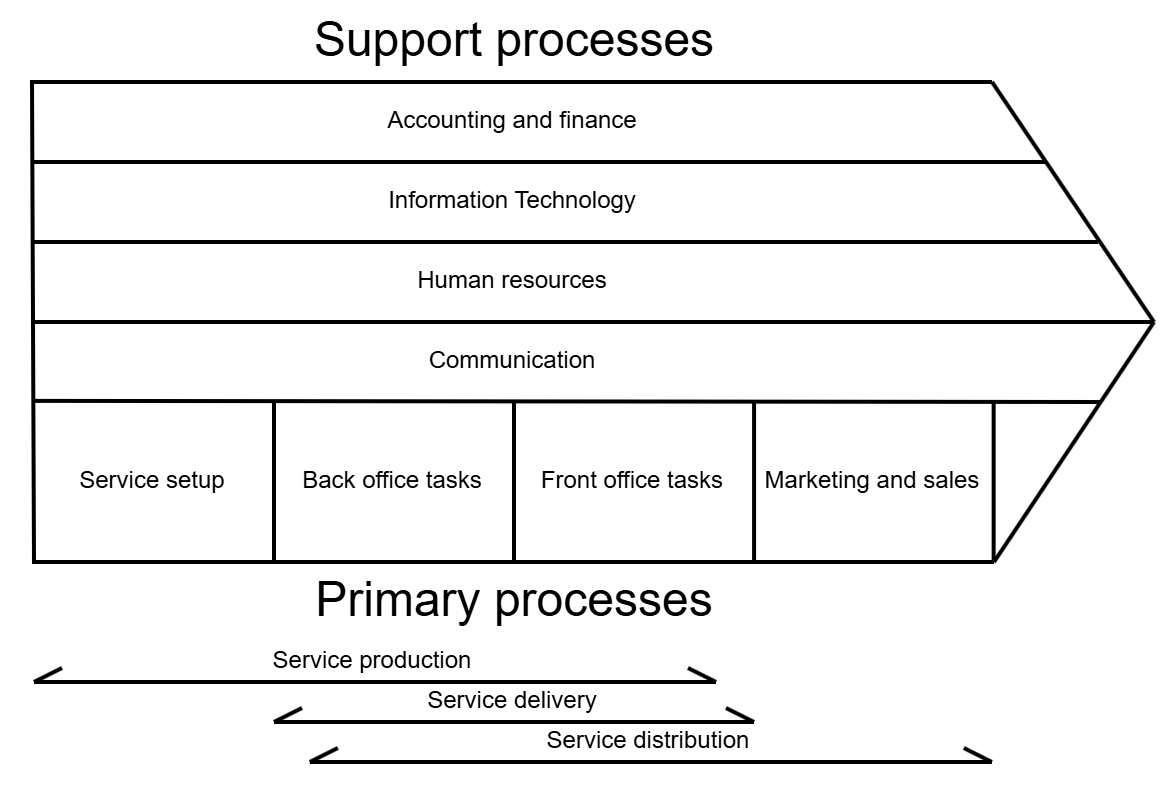
\includegraphics[width=0.5\linewidth]{images/bis13.png}
    \caption{New Porter}
\end{figure}

\subsubsection{Post-hoc methods}
Post-hoc explainability methods aim to make predictions from existing machine learning models interpretable. 
These can be categorized as:
\begin{itemize}
    \item \textit{Model specific}: supports explainability constraints based on the learning algorithm and the internal structure of the model.
    \item \textit{Model agnostic}: nnvolves applying pairwise analysis of model inputs and predictions, making the explanation applicable regardless of the model type.
    \item \textit{Global}: provides an explanation that covers all units in the dataset, offering insights into the entire model's behavior.
    \item \textit{Local}: 0ffers an explanation for a specific subset of data, focusing on a particular kind of dataset or input.
\end{itemize}
\noindent Common post-hoc XAI approaches includes:
\begin{itemize}
    \item \textit{Feature importance}: assigns an importance value to each variable based on how much it influences the prediction. 
    \item \textit{Surrogate models}: simplifies a complex model by approximating it with a more explainable, interpretable model.
    \item \textit{Rule-based}: uses if-then rules to express combinations of input features and their activation values.
    \item \textit{Saliency maps}: highlights the important input pixels or features that have the most significant impact on the prediction.
\end{itemize}

\paragraph*{Benefits}
The benefits of XAI are: 
\begin{itemize}
    \item \textit{Justify}: helps explain and justify the system's behavior, allowing users to detect unknown vulnerabilities and flaws.
    \item \textit{Improve}: facilitates the improvement of model performance, debugging, and verification by applying structured engineering approaches.
    \item \textit{Control}: ensures better control and supervision of the algorithm, guaranteeing its proper usage and compliance with standards.
    \item \textit{Discover}: enables the discovery of potential biases or faults in the model by comparing its reasoning, helping assess its validity and reliability. 
        It also identifies the most influential factors behind predictions.
\end{itemize}

\subsubsection{Reponsible AI}
Responsible AI encompasses various sub-disciplines, including: explainable AI, human-centered AI, compliance, ethical AI, secure AI, and interpretable AI. 

The goal of responsible AI is to develop AI systems that are not only effective but also transparent, ethical, secure, and compliant with established standards, ensuring they are used responsibly in real-world applications.